\chapter{Introduction}\todo[inline]{modify chapter headings as required}

\section{Background to the problem}

Normal `sentence case' is preferred for all headings, don't capitalise each word (e.g.~as above, not ``Background to the Problem").

\subsection{Brief Bib\TeX\ tips}

To illustrate the difference between \verb|\citet| and \verb|\citep|, and how to cite an honours thesis:
\begin{itemize}
  \item \citet{Smith} studied the problem of writing templates, but
  \item many examples of citing honours theses exist in the literature \citep{Smith}.
\end{itemize}
Refer to a standard as follows \citep{ISO3382-2}. With multiple authors make sure you separate each of the author's names with `and' \citep{BookExample}. Note the following features in this reference to \citet{vonKarman}:
\begin{itemize}
  \item multiple authors separated by `and' in the {\tt .bib} file,
  \item special character (\'a)
  \item compound surname needs to be contained in \{\}
  \item use of `DOI' reference (digital object identifier)  
\end{itemize}

More information can be found at \url{http://www.bibtex.org/} and some good examples at \url{https://verbosus.com//bibtex-style-examples.html}.

\subsection{Tables and figures}

Table~\ref{tab:demo} illustrates a simple table, while Figure~\ref{fig:demo} illustrates a figure with subfigures.



\begin{table}[htbp]
  \centering
  \begin{tabular}{ccl}
    \hline
    \textbf{Sample} & \textbf{Maximum recorded} &  \textbf{Failure location} \\
    \textbf{}		& \textbf{load (kN)}		&  \textbf{} \\
    \hline
    $C$    &  197.0  &  Top machined face     \\
    $U_1$  &  199.2  &  Above concrete        \\
    $U_2$  &  221.4  &  Top machined face     \\
    $W_1$  &  199.0  &  Middle machined face  \\
    $W_2$  &  197.0  &  Bottom machined face  \\
    \hline
    \end{tabular}
  \caption{A sample table.}
  \label{tab:demo}
\end{table}

\begin{figure}[htbp]
\centering
	\subfigure[Left subfigure.]{
        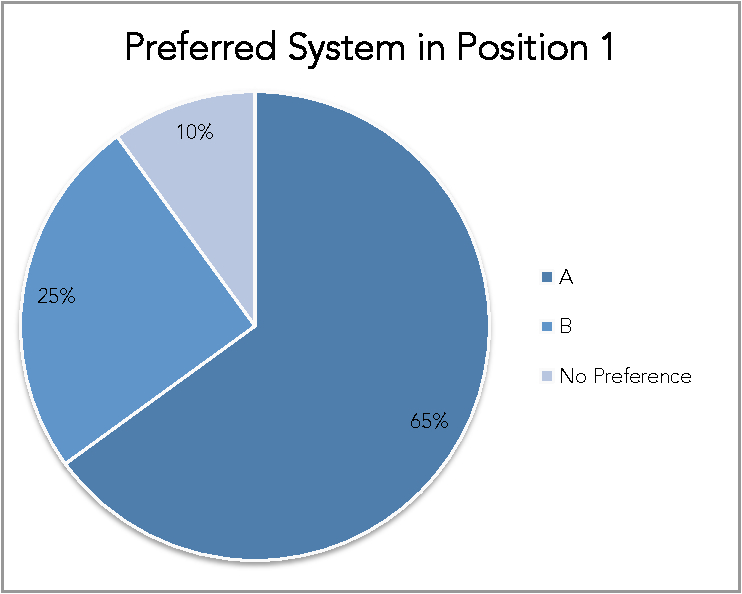
\includegraphics[width=.35\textwidth]{Pos1.pdf}
        \label{fig:Pos1}}
 \quad\quad
	\subfigure[Right subfigure.]{
        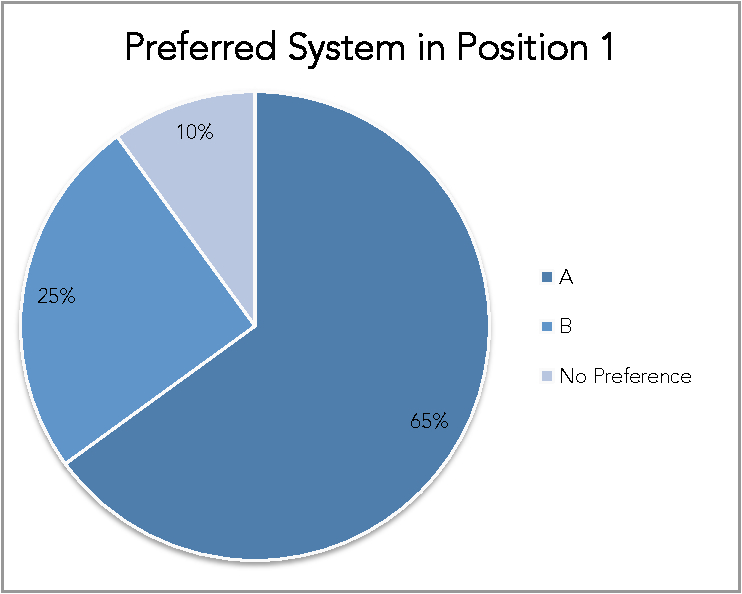
\includegraphics[width=.35\textwidth]{Pos1.pdf}
        \label{fig:Pos2}}
   \caption{A sample two part figure using the {\tt subfigure} package.}
  \label{fig:demo}
\end{figure}


\section{Problem statement}

\section{Project scope}
